\chapter{Code structure}

I created three Gradle projects, backend, frontend and common. When building the application, the common code is compiled into both layers. Layers can thus share knowledge of the same classes, but don't need to import one another, they can be distributed as completely separate packages.

\section{Network communication}
The application was built in such a way that any current and future communication between the server and client can be made using an RFC 6455-compliant\cite{RFC6455} WebSocket provided by the server. This allows asynchronous, thread-safe communication between the two parties without being bound by packet timing. This approach also supports a "multiple clients, single server" architecture.

\subsection{Websocket usage}
Websocket communication is usually started by a client pinging a target address where a server resides. The initiating message is a handshake that must contain the host, port, resource name, and a flag showing whether the connection is secure. Secure connections must also include a TLS handshake. If the server replies, a TCP\footnote{Transmission Control Protocol, a connection-oriented protocol, used by much of today's internet traffic} connection is established -- a two-way tunnel for sending further messages with low delay. The connection has a set of possible states. There can only ever be one "connecting" socket (one that is being established but is not yet ready for data) between any given pair of machines, and sockets may fail. It's worth to keep in mind that a failed socket may drop data when disconnecting; text still in transit will not be re-sent.

Each packet, called a frame in this context, may be a data frame or a control frame. Control frames include "ping", "pong" and "close". Data frames can be used to transit text or binary data. The main noticeable difference from a standard TCP endpoint is the URI scheme: "ws://" in this case. Arbitrary data may be serialised~(see \ref{serialise}) to a data interchange format, such as JSON (JavaScript Object Notation) or YAML (Yet Another Markup Language). Text is highly compressible, so a properly set up websocket gets more efficient with larger payloads.

Websockets have several advantages applicable to this project: they're connections that are easy to keep alive and may transfer data in large batches. Setup is also easy, it's compatible with HTTP and most languages have robust libraries to manage sockets. They're slightly slower than a simple TCP connection due to their overhead; this not a problem in this case, as the ordering and timing of messages is not critical. Decoupled messages are also better for using asynchronous structures.

\subsection{Ktor-specific solutions}

In Ktor, a socket server is created by overriding the \verb|Application.configureRouting()| method. An endpoint can be made by using "webSocket" in place of an HTTP verb, such as "get" or "post"; in my case, it's available at \verb|ws://host:port/control|. The appropriate Ktor plugin must also be installed from code and can be configured here; options include the timeout and ping periods, and the selection of a content conversion strategy. I used Json with serialised class discriminators to send custom control messages. These are simple data classes in a two-level inheritance hierarchy, and replace string input validation with compile-time guarantees for the type of data transmitted.

\label{control-msg}
\begin{figure}[!ht]
    \centering
    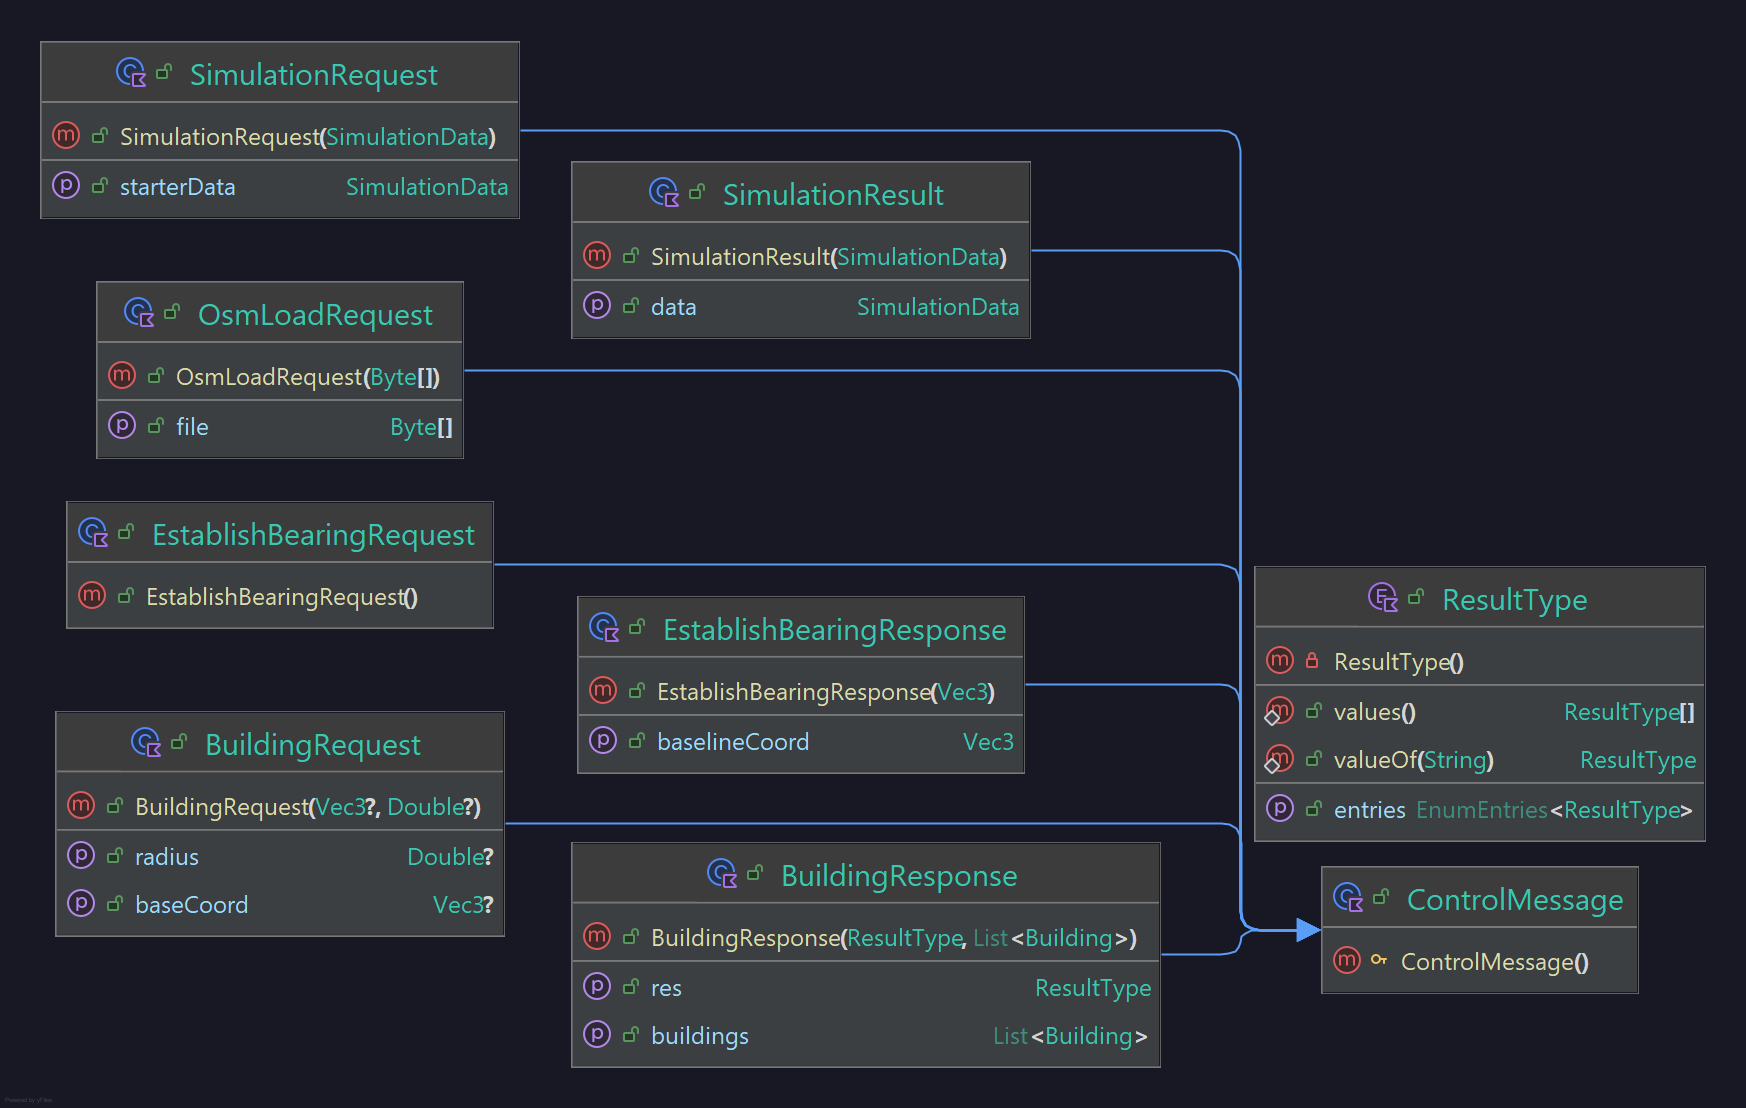
\includegraphics[width=140mm, keepaspectratio]{images/control-messages.png}
    \caption{The control messages used for communication}
\end{figure}

The endpoint has an implicit "incoming" attribute. This is a Kotlin ReceiveChannel, which is coroutine-based and helps avoid busy waiting\footnote{constantly retrying an operation (\eg~getting data from a usually empty container), this is generally wasteful} by suspending the current program flow until a message can actually be retrieved. Sending a response is done by calling \verb|sendSerialized()|, which puts data into the "outgoing" SendChannel. As long as the socket is kept open using pings, these channels may be queried continuously.

The SocketServer/SocketClient classes are responsible for the actual connections, they're treated as singletons in their respective software layers. When a message is received on either end, a map of type-function\footnote{functions are first-class citizens in Kotlin} pairs is queried, and the corresponding operation is run using a coroutine, provided it is listed. This flaunts the Open-Closed Principle in object-oriented programming, defined by Bertrand Meyer\cite{OOSC-OCP} as follows: \say{Modules should be both open and closed. [\ldots] A module is said to be closed if it is available for use by other modules. This assumes that the module has been given a well-defined, stable description.} While the message class itself is open to extension, any modification requires changing the list of callback functions. I found this to be an acceptable trade-off, as it protects against typos, missing fields and the processing of unknown messages.
The server keeps a list of all connected clients and treats them as subscribers, sending every response to all of them; one backend instance can service multiple clients.

\label{file-upload}
The client may send a protocol buffer file through the \verb|/pbf_file| POST endpoint to overwrite the current database with a different region of the globe. Data is loaded as described in section~\ref{pbf-loading}. This is the single message that does not use websockets for transmission.

\section{The database}

I chose SQLite as my database engine. It's lightweight, decently fast, and self-contained. The theory is that the .db file may be used like a video game save if needed, since deep copies can be mode by duplicating the file. Most other database engines are unsuitable for this, because their data may span multiple files or even systems. SQLite has no automatic backups -- losing this program's database is not a concern, though, as it can be rebuilt in seconds. For transactions, the standard ACID (atomicity, consistency, isolation, durability) principles are followed.

\label{pbf-loading}
The database is created when loading a new PBF dataset, and can be read unlimited times until a new file is presented. The program spawns a PBF iterator from the osm4j library and reads every element into an OsmStorage object. Nodes and ways are read unconditionally, as relations must reference them to hold any meaningful data. Out of every category, elements with the \verb|highway| or \verb|building| tag are collected, their child elements retrieved and dumped into the database. After this process, the on-CPU storage object is purposefully thrown away and cleaned up due to the high number of unused nodes.

I ended up going with a very simple data structure of just two tables, Buildings and Roads. Both tables have osm\_id, tags and ways columns, and buildings include additional information about their location, OSM element type, as well as a capacity, calculated as a function of their area and height. Some buildings have a "height" tag that's specified in meters, or a "levels" tag counting its floors. If none of these is present, I calculate the value as if there was only one storey. Capacity is used by the random selection algorithm while simulating to weigh the options. Roads are stored as simple splines of one or more serialised ways, with their separate tags also stored (if they have any). This does not encode width information as per OSM guidelines.

The OSM tags take up the most space in the database, as they're simple strings that can't be reasonably simplified. Since the key-value pairs are unique most of the time, I found no real gains in creating a foreign key structure for them and instead used a JSON serialiser. Later editions of the software could have a hybrid solution: a lookup table for common values, and simple string storage for all others.

\subsection{Data access}

Database communication is handled by the DatabaseAccess singleton. All methods are independent of the engine being used, so the database connection string could be swapped to use any other engine supported by Exposed. Queries are serialisable transactions, which mostly prevents read-write collisions in case the user requests to load a new dataset while the current one is still being queried. Kotlin natively supports Sequences, a list type that can produce items while it's being iterated. I made use of this to send building data to the socket in smaller chunks, before the whole transaction is done, reducing crashes and improving performance. Exposed provides a DSL-specific transaction block, which runs all contained code in a database context, automatically dropping changes if any errors are raised. If the transaction block would ever freeze, incomplete data may be sent, but the program does not have to terminate.

\section{Common classes}

I made the following utility classes in the common project. \begin{itemize}
    \item \textbf{SerializeableNode/Way/Tag} -- Data classes explicitly annotated as @Serializable for Ktor, they wrap their respective osm4j types. Tags are expressed as "key=value" strings.
    \item \textbf{Vec3} -- A three-dimensional vector class with basic arithmetic methods, and Doubles instead of Floats. These are used throughout the program to maintain higher precision when using real-world coordinates.
    \item \textbf{Building, Road} -- The runtime equivalents of the database records. The frontend can't see the database structure, only these representations. They also function as Data Access Objects (DAOs) for Exposed.
    \item \textbf{Agent} -- A person in the city and simulation. They have a pre-set speed and age group. Their precise location in the world is also stored.
    \item \textbf{ObservableMap} -- A typical Kotlin MutableMap, extended with callbacks for any changes that occur (for example, adding an item).
    \item \textbf{ControlMessage (and inheriting classes)} -- A simple explicitly serialisable class with predefined fields; this is how I ensured that every websocket message contained the expected data. See \ref{control-msg}
\end{itemize}

\label{serialise}
Exposed supports custom columns, which I used to convert each Vec3 instances to a VARCHAR\footnote{variable length character array, it can store arbitrary text up to its length limit, only using the necessary number of bytes} type in SQL. This is type-safe when reading or writing, conversion happens automatically.
\begin{lstlisting}[caption=Custom column type in JetBrains Exposed]
    object Vec3ColumnType : ColumnType<Vec3>() {
    override fun sqlType(): String = "VARCHAR(50)"
    override fun valueFromDB(value: Any): Vec3 {
        return when (value) {
            is String -> Vec3.fromString(value)
            else -> ...}} ... }
\end{lstlisting}

\section{The frontend}

\begin{figure}[!ht]
    \centering
    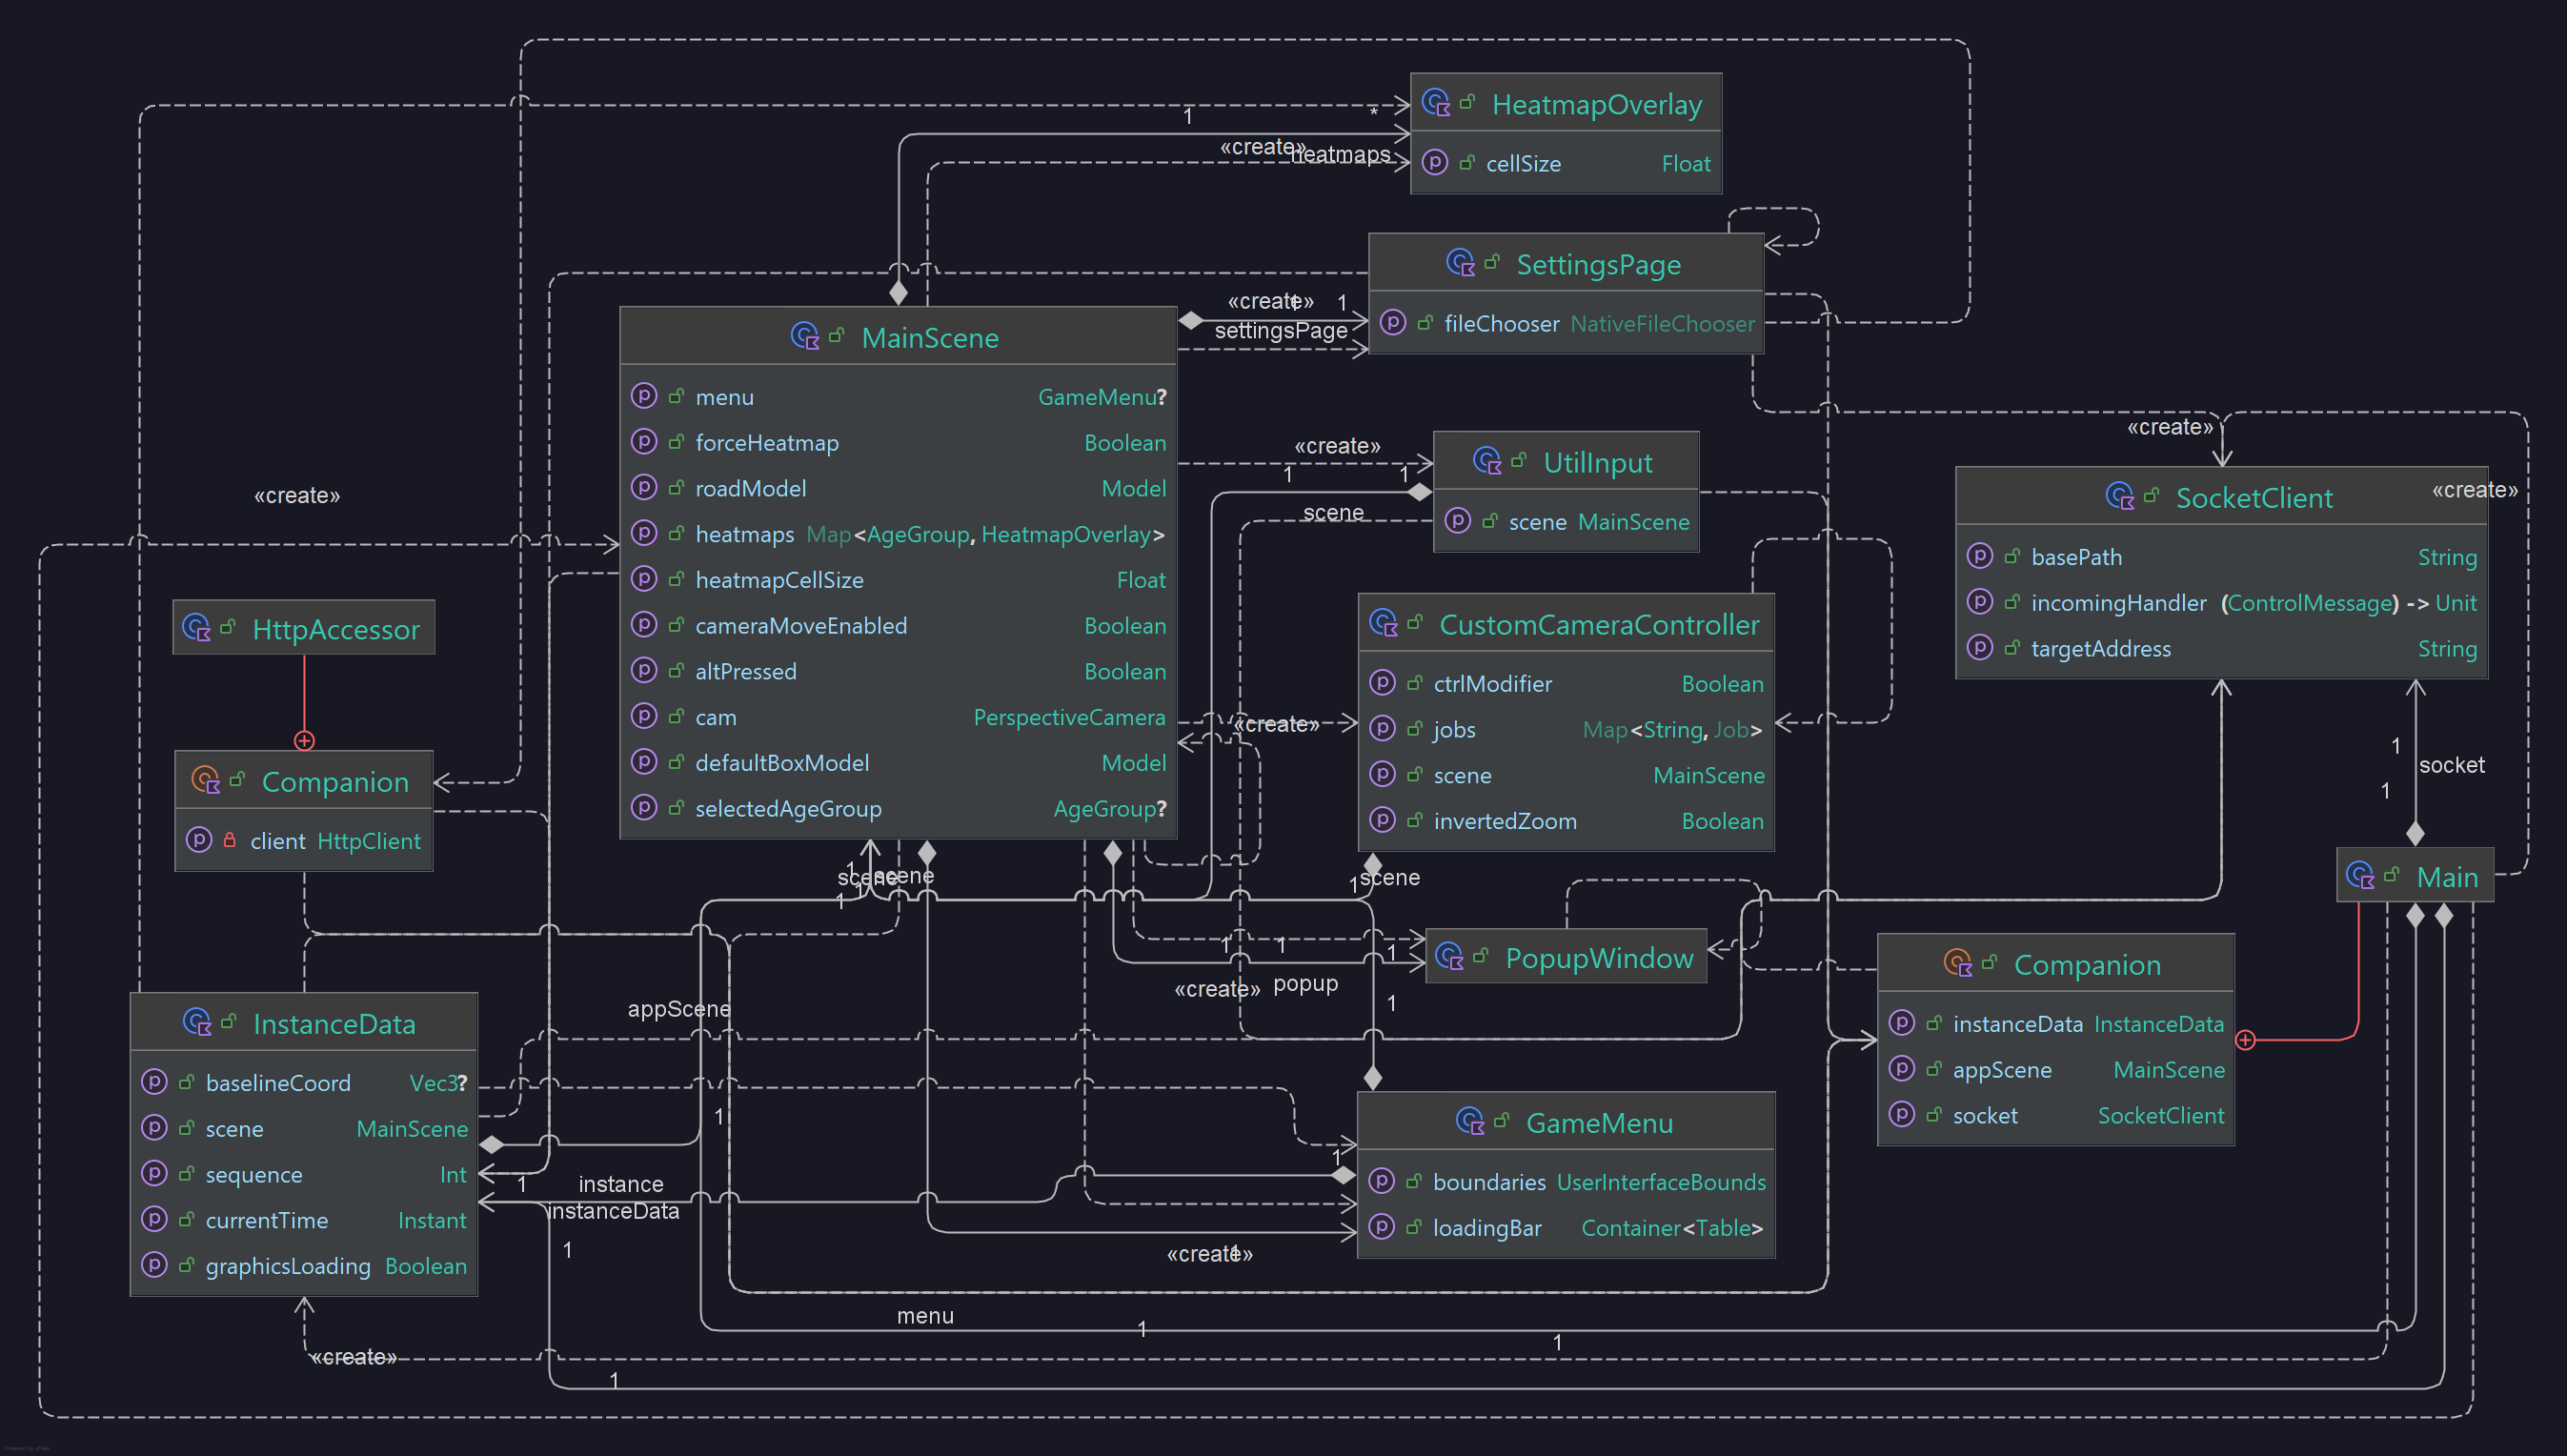
\includegraphics[width=140mm, keepaspectratio]{images/frontend-classes.png}
    \caption{Diagram of the most important classes on the frontend}
\end{figure}

The client project takes a slightly more centralised approach. It's a libGDX application, with a \verb|MainScene| class as the focus. Input controllers and other data are imported directly into this class. LibGDX variables utilise Kotlin's lateinit feature as they can only be assigned once there is a current graphics context, in the \verb|create()| function.

The \verb|InstanceData| class handles everything not directly related to graphics and OpenGL functions; it orchestrates requests, handles incoming messages, gives commands to the main scene and its menus. All queried objects are put into an ObservableMap, and puts automatically trigger the corresponding function to insert the object into the scene.

%TODO